\documentclass[12pt]{report}
%\documentclass[12pt,twoside]{report}
\usepackage[utf8]{inputenc}
%\usepackage{amsmath}
%\usepackage{amsfonts}
%\usepackage{amssymb}
\usepackage{caption}
\usepackage{subcaption}
\usepackage{graphicx}
\graphicspath{ {Images/} }
\usepackage{xcolor}
\usepackage{listings}


\lstdefinestyle{DOS}
{
	backgroundcolor=\color{black},
	basicstyle=\scriptsize\color{white}\ttfamily
}


\makeatletter
\def\@@acrodef{\@ifstar\@acrodefs\@acrodef}
\newtoks\acro@list
\newcommand{\@acrodef}[2]{%
	\global\acro@list=\expandafter{\the\acro@list\@elt{#1}{#2}}%
	\global\@namedef{acro@#1}{n{#1}{#2}}}
\newtoks\acro@resetlist
\newcommand{\@acrodefs}[2]{%
	\global\acro@resetlist=\expandafter{\the\acro@resetlist\@elt{#1}}%
	\@acrodef{#1}{#2}}
\def\acro@doresetlist{\begingroup
	\def\@elt##1{\expandafter\expandafter\expandafter
		\acro@reset\csname acro@##1\endcsname}\the\acro@resetlist\endgroup}
\def\acro@reset#1#2#3{\global\@namedef{acro@#2}{n{#2}{#3}}}
\newcommand{\acro}[1]{\expandafter\expandafter\expandafter
	\use@acro\csname acro@#1\endcsname}
\def\use@acro#1#2#3{\ifx n#1
	#3 (#2)\global\@namedef{acro@#2}{o{#2}{#3}}%
	\else
	#2%
	\fi}
\newcommand{\listofacronyms}[1][tabular]{%
	\begingroup\def\@elt##1##2{##1&##2\\}%
	\@ifundefined{chapter}{\section*}{\chapter*}{\listacronymname}
	\noindent\begin{#1}{@{}p{6em}p{\dimexpr\columnwidth-2\tabcolsep-6em\relax}@{}}
		\the\acro@list
	\end{#1}\endgroup}
\providecommand\listacronymname{List of acronyms}
\newenvironment{acronyms}{\let\acrodef\@@acrodef}{}
\newenvironment{acronyms*}{\let\acrodef\@@acrodef}{\listofacronyms}
\def\g@preto@macro#1#2{\toks0=\expandafter{#1}%
	\toks2={#2}\xdef#1{\the\toks2 \the\toks0 }}
\@ifundefined{chapter}
{\g@preto@macro\section\acro@doresetlist}
{\g@preto@macro\chapter\acro@doresetlist}
\makeatother

%\usepackage[a4paper,width=150mm,top=25mm,bottom=25mm]{geometry}

\usepackage{fancyhdr}
\pagestyle{fancy}
\usepackage{fvextra}

\fancyhead{}
\fancyhead[RO,LE]{Thesis Title}
\fancyfoot{}
\fancyfoot[LE,RO]{\thepage}
%\fancyfoot[LO,CE]{Chapter \thechapter}
%\fancyfoot[CO,RE]{Author Name}

%\usepackage{biblatex}
%\addbibresource{references.bib}




%TEXT\parencite[see][p10]{latexcompanion}
%TEXT\parencite[compare][]{knuthwebsite}
%TEXT\parencite[e.g.][page 300]{einstein}

\title{
	{MeerKat Operator Manual}\\
	{\large SARAO}\\
	\vspace{1.5cm}
	{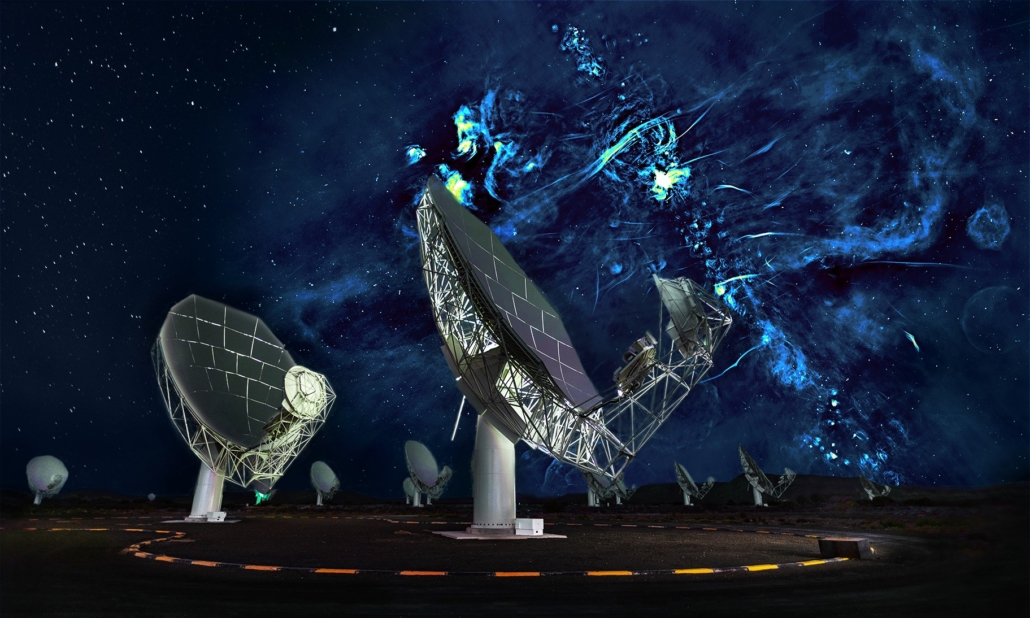
\includegraphics[width=16cm]{cover.jpg}}
}
\vspace{1.5cm}
\vspace{1.5cm}
\vspace{1.5cm}
\vspace{1.5cm}
\vfill
\author{Telescope Operators}
\date{}

\begin{document}
\maketitle
 
 
 \chapter*{Preface}

This manual is designed to help new users (i.e Students,Visitors, ) of the MeerKat Radio Telescope\cite{} to link and to undestand basic operational procedures\cite{}, and scientific procedures\cite{} that are being used to carry out scientific observations.  The complexity of the instrument requires many software interfaces for instrument setup, scheduling, monitorig and maintenace management. \\
\\
 Most of the operational terminologies and commands can only be understood by people in the operations and commissioning divisions of SARAO, thus the document bridges that gap.  The sientific community is more interested in underlying scientific methods, validation and qualification procedures that are the ultimate goal of all the operational activities.  
 
 \chapter*{Naming Convenctions }
 The following typographical rules and standards \cite{standard1} \cite{standard2} have been adopted for this manual:
 \begin{itemize}
 	\item {} Units
 	\item {} Names of servers and computers
 	\item {} Names of software packages
 	\item {} Names of software programs
 	\item {} Command line/terminal command e.g 
 	\begin{lstlisting}[style=DOS]
 	ssh kat@obs.mkat.karoo.kat.ac.za
 	\end{lstlisting}
 	\item {} Windows command
 	\item {} Filename, e.g
 	\item {} Program option
 	\item {} Acchronyms
 	\item {} Placeholder for changeable parameters
 	\item {} Optional parameter,
 	\item{ } List of possible commands or parameters
 	
 \end{itemize}
 \begin{acronyms*}
 	\acrodef{	ABL	}{	Allocated Baseline	}
 	\acrodef{	Ac	}{	Critical Availability	}
 	\acrodef{	ADR	}{	Architecture Design Review	}
 	\acrodef{	AGN	}{	Active Galactic Nuclei	}
 	\acrodef{	Ai	}{	Inherent Availability	}
 	\acrodef{	AOR	}{	Annual Operating Requirement	}
 	\acrodef{	AR	}{	Acceptance Review	}
 	\acrodef{	BOM	}{	Bill Of Material	}
 	\acrodef{	CA	}{	Criticality Analysis	}
 	\acrodef{	CDR	}{	Critical Design Review	}
 	\acrodef{	DDR	}{	Detail Design Review	}
 	\acrodef{	D-Level	}{	Deport Level	}
 	\acrodef{	DLM	}{	Depot Level Maintenance	}
 	\acrodef{	FAT	}{	Factory Acceptance Tests	}
 	\acrodef{	FMEA	}{	Failure Modes and Effects Analysis	}
 	\acrodef{	FMECA	}{	Failure Modes, Effects and Criticality Analysis	}
 	\acrodef{	FPGA	}{	Field Programmable Gate Array	}
 	\acrodef{	FRACAS	}{	Failure Reporting and Corrective Action System	}
 	\acrodef{	GHz	}{	Giga Hertz	}
 	\acrodef{	GUI	}{	Graphical User Interface	}
 	\acrodef{	HartRAO	}{	Hartbeeshoek Radio Astronomy Observatory	}
 	\acrodef{	Hrs	}{	Hours	}
 	\acrodef{	I-Level	}{	Intermediate Level	}
 	\acrodef{	ILM	}{	Intermediate Level Maintenance	}
 	\acrodef{	ILOR	}{	Intended Learning Outcomes Report	}
 	\acrodef{	ILS	}{	Integrated Logistic Support	}
 	\acrodef{	ISO	}{	International Standards Organisation	}
 	\acrodef{	KAT-7	}{	Karoo Array Telescope, 7 array	}
 	\acrodef{	Kg	}{	Kilogram	}
 	\acrodef{	Km	}{	Kilometer	}
 	\acrodef{	L3/4/5	}{	Level 3/Level 4/Level 5	}
 	\acrodef{	LEMP	}{	Logistic Engineering Management Plan	}
 	\acrodef{	LRU	}{	Line Replaceable Unit	}
 	\acrodef{	LSA	}{	Logistic Support Analysis	}
 	\acrodef{	MBL	}{	Manufacturing Baseline	}
 	\acrodef{	MSCDR	}{	Media Selection \& Curriculum Development Report	}
 	\acrodef{	MSP	}{	Maintenance \& Support Plan	}
 	\acrodef{	MTBCF	}{	Mean Time Between Critical Failures	}
 	\acrodef{	MTBF	}{	Mean Time Between Failures	}
 	\acrodef{	MTTRc	}{	Mean Time To Repair Critical	}
 	\acrodef{	MTTRi	}{	Mean Time To Repair Inherent	}
 	\acrodef{	NQF	}{	National Qualification Framework	}
 	\acrodef{	OEM	}{	Original Equipment Manufacturer	}
 	\acrodef{	O-Level	}{	Organisational Level	}
 	\acrodef{	OLM	}{	Organisational Level Maintenance	}
 	\acrodef{	OTLR	}{	Operator Task List Report	}
 	\acrodef{	PBL	}{	Product Baseline	}
 	\acrodef{	PBS	}{	Physical Breakdown Structure	}
 	\acrodef{	PC	}{	Printed Circuit	}
 	\acrodef{	PDR	}{	Preliminary Design Review	}
    	\acrodef{PHS and T}{Packaging, Handling, Storage and Transportation	}
    \acrodef{	PPPM	}{	Preparation, Preservation, Packaging \& Marking	}
    \acrodef{	PPPR	}{	Personnel Performance Profile Report	}
    \acrodef{	PRR	}{	Production Readiness Review	}
    \acrodef{	PSS	}{	Product Supplier Support	}
    \acrodef{	QBL	}{	Qualification Baseline	}
    \acrodef{	RAM	}{	Reliability, Availability, Maintainability	}
    \acrodef{	RBL	}{	Requirements Baseline	}
    \acrodef{	Relc	}{	Reliability Critical	}
    \acrodef{	Reli	}{	Reliability Inherent	}
    \acrodef{	RF	}{	Radio Frequency	}
    \acrodef{	RFI	}{	Radio Frequency Interference	}
    \acrodef{	RM	}{	Rotation Measures	}
    \acrodef{	RR	}{	Requirements Review	}
    \acrodef{	RTS	}{	Receptor Test System	}
    \acrodef{	S and TE	}{	Support and Test Equipment	}
    \acrodef{	SAQA	}{	South African Qualifications Authority	}
    \acrodef{	SEMP	}{	System Engineering Management Plan	}
    \acrodef{	SKA	}{	Square Kilometer Array	}
    \acrodef{	S-Level	}{	Supplier Level	}
    \acrodef{	SLM	}{	Supplier Level Maintenance	}
    \acrodef{	SNR	}{	Supernova Remnants	}
    \acrodef{	SRU	}{	Shop Replaceable Unit	}
    \acrodef{	TBD	}{	To Be Determined	}
    \acrodef{	TRR	}{	Test Readiness Review	}
    \acrodef{	TSR	}{	Training Survey Report	}
    \acrodef{	TTLR	}{	Technical Task List Report	}
    \acrodef{	vs	}{	Versus	}
\end{acronyms*}
 
% \section{A}
% 
% \acro{GEOAA}
% 
% \acro{IMO}
% 
% \acro{IMO}
% 
% \acro{GEOAA}
% 
% \acro{OP}
% 
% \section{B}
% 
% \acro{OP}
 
% \listofacronyms
 
 %\chapter*{Dedication}

% \renewcommand{\headrulewidth}{0.4pt}
% \renewcommand{\footrulewidth}{0.4pt}
% \chapter*{Declaration}
 
% \chapter*{Acknowledgements}
 
  \listoffigures
  
 \tableofcontents
 \chapter{Introduction}
 \section{Int}
see \textbf{Figure}:\ref{fig:three graphs}
\begin{figure}
	\centering
	\begin{subfigure}[b]{0.3\textwidth}
		\centering
		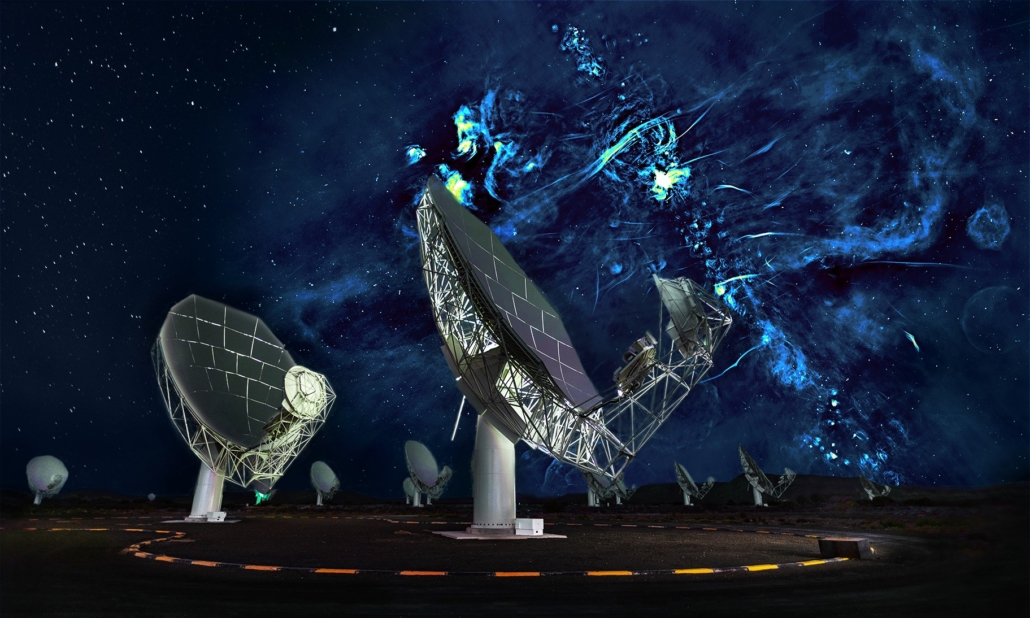
\includegraphics[width=\textwidth]{cover.jpg}
		\caption{$y=x$}
		\label{fig:y equals x}
	\end{subfigure}
	\hfill
	\begin{subfigure}[b]{0.3\textwidth}
		\centering
		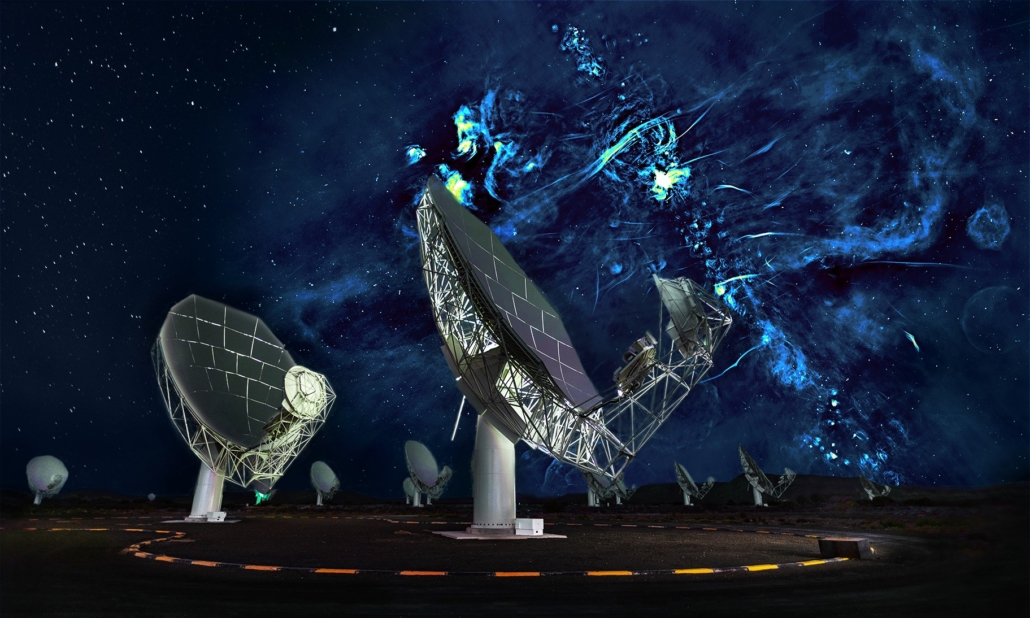
\includegraphics[width=\textwidth]{cover.jpg}
		\caption{$y=3sinx$}
		\label{fig:three sin x}
	\end{subfigure}
	\hfill
	\begin{subfigure}[b]{0.3\textwidth}
		\centering
		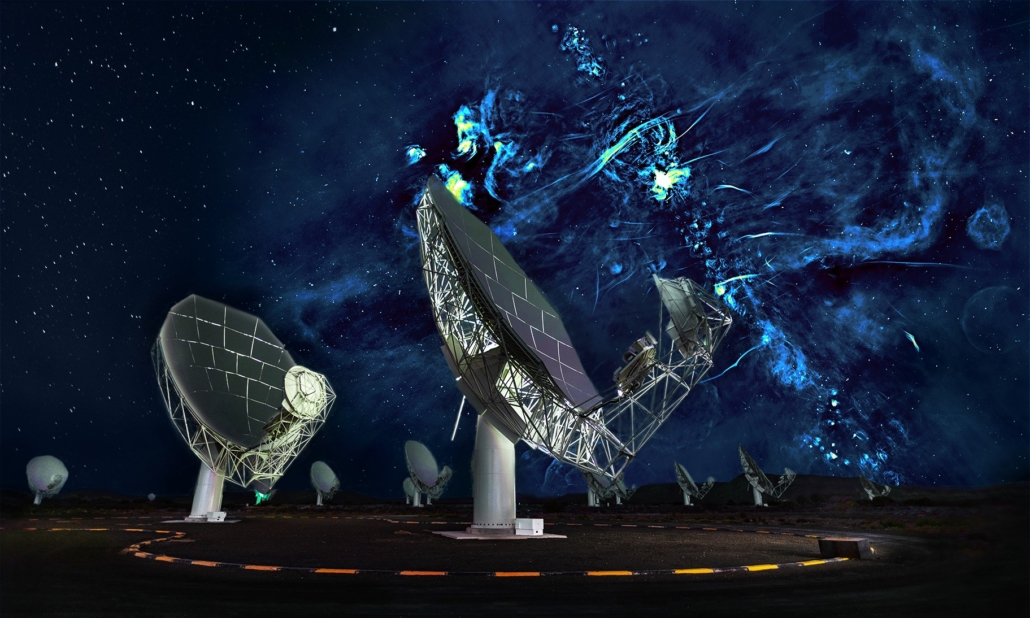
\includegraphics[width=\textwidth]{cover.jpg}
		\caption{$y=5/x$}
		\label{fig:five over x}
	\end{subfigure}
	\caption{Three simple graphs}
	\label{fig:three graphs}
\end{figure}

  \chapter{Instrument Calibration Procedures}
 \section{Receiver System Tests (RTS) and Calibration}

\section{Cable Delay Calibration}
\subsection{Band Pass Calibration}
\section{Phase-up and Phase Down}
\section{Pointing Calibration}
\subsection{Single Dish Pointing}
\subsubsection{Pointing Check}
\subsubsection{Interfrometric Pointing}
\subsubsection{AP Motion Profilers}
\section{Holography Test}


\section{Digitiser attenuation levels}
\section{System Sychoronisation}

\subsection{Digitiser Master Controller}
\subsection{Digitiser Synchronisation}
\subsection{Aantenna Control Unit Synchronisation}



	
 
  \chapter{Safety Procedure}
 \section{ Operational Safety Procedure}

 
 \chapter{System Settings Procedures}
 


\section{Moving Skarabs}


\textbf{WARNING}:\textit{ do not try to move the skarabs right after stopping or starting a subarray. The SKARABs need a couple of minutes to restart. Otherwise, they will not be found by the script, and will be left behind on the unwanted cmc.}\\

\subsection{CMC IP addresses}
The IP addresses for different machines are:
\begin{itemize}


	\item[] \server{cmc1: 10.103.254.1} and name: \server{cmc1.cbf.mkat.karoo.kat.ac.za}
\item[] \server{cmc2: 10.103.254.3} and name: \server{cmc2.cbf.mkat.karoo.kat.ac.za}, 

\item[] You can use the IP addresses or hostnames interchangeably (whichever you prefer) 


\item[] The cbf\_support repository is on git. You can clone it from:\\
git clone \url{https://github.com/ska-sa/cbf_support}
\end{itemize}
\subsection{Check the number of SKARABS}
In order to check the number if SKARABS are available in the CMC use the following
commands on the obs machine before attempting to move them. There should be about 220(as at 2020-01-06, but more will come) if they were all moved. If there are less, wait a couple
of minutes for them to restart.

\begin{lstlisting}[style=DOS]
kcpcmd -t 10 -s cmc1.cbf.mkat.karoo.kat.ac.za:7147 resource-list | grep "up$" | wc -l
\end{lstlisting}
(this will give you the number of skarabs available on cmc1.) 
\begin{lstlisting}[style=DOS]
kcpcmd -t 10 -s cmc2.cbf.mkat.karoo.kat.ac.za:7147 resource-list | grep "up$" | wc -l
\end{lstlisting}
(this will give you the number of skarabs available on cmc2.) \\

\subsection{Moving SKARABS}
If moving to cmc1 use -m cmc1:
\begin{lstlisting}[style=DOS]
./usersnfs/cbf_support/./cmc_manage_skarabs.py -m cmc1 -a 5 6 7 8 9 10 11 12 13 14 15 16 17 18 
 -k cmc1 cmc2
\end{lstlisting}
If moving to cmc2 use -m cmc2:
\begin{lstlisting}[style=DOS]
./usersnfs/cbf_support/./cmc_manage_skarabs.py -m cmc2 -a 5 6 7 8 9 10 11 12 13 14 15 16 17 18  -k cmc1 cmc2
\end{lstlisting}




This will connect to all the switches, discover which skarabs are currently online on the various ports, and move them to the requested master controller (-m switch).



\section{Global Synchronisation}

This script seeks to synchronize all digitisers to the Digitiser Master Controller so that signal/data coming into the correlator is in sync and correlates. 
\begin{itemize}
\item{} Ensure epoch sync on all usable digitisers (all bands) is done for the day
\item{} In the GUI, verify that all subarrays are inactive:
\begin{lstlisting}[style=DOS]
ssh kat@obs.mkat.karoo.kat.ac.za
run /home/kat/katsdpscripts/utility/global_sync.py
--observer= name --proposal-id=OPS-23

\end{lstlisting}



\item To check that all digitisers are synced and have the same epoch time, in the
same ipython session
\begin{lstlisting}[style=DOS]
ipython
import katuilib
configure()
kat.report_sensors('epoch','all')
\end{lstlisting}

\item Three ways to check time remaining for the next global sync
\begin{itemize}


\item [$\circ$] Check the Next Global Sync from the active subarray in the GUI (see \textbf{Figure}~\ref{fig:image115}). This gives
indication on what is the time remaining before the next global sync is
done.
\begin{figure}[H]
	\centering
	%\includegraphicsdpi{100}{}{bur1.png}     
	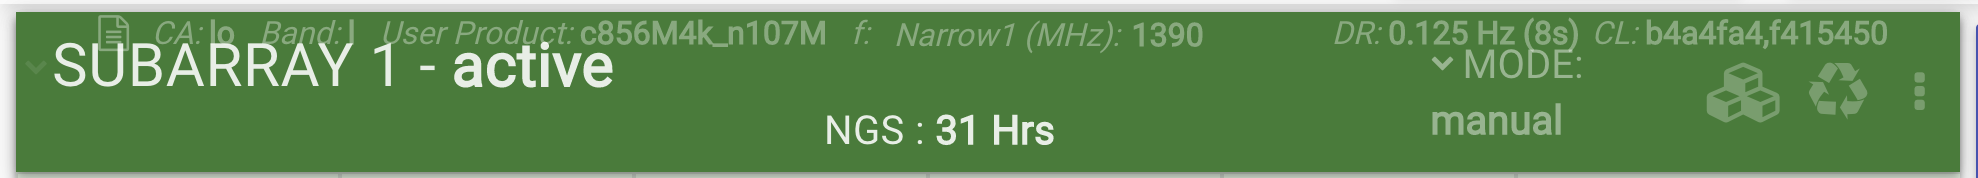
\includegraphics[scale=0.46]{Chapters/images/image115.png}
	
	%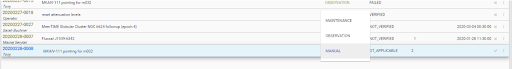
\includegraphics[resolution=100]{bur1.png}
	\caption{Global sync time remaining alert on the GUI }
	\label{fig:image115}
\end{figure}
\item [$\circ$] From the sensor list by typing \sensor{remaining} as shown in \textbf{Figure}~\ref{fig:image121}.
\begin{figure}[H]
	\centering
	%\includegraphicsdpi{100}{}{bur1.png}     
	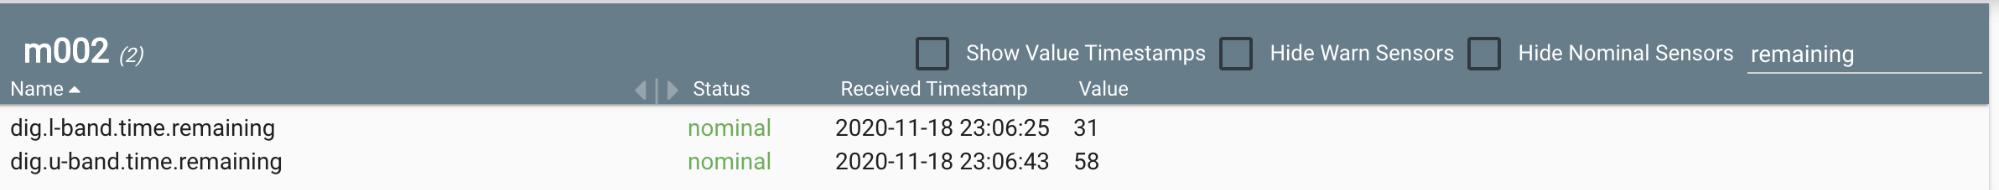
\includegraphics[scale=0.23]{Chapters/images/image121.png}
	
	%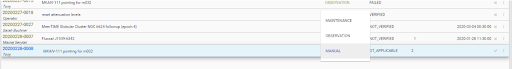
\includegraphics[resolution=100]{bur1.png}
	\caption{Global sync time remaining alert in sensor list}
	\label{fig:image121}
\end{figure}
\item [$\circ$] On IRC there is a reminder that reminds when to run a Global sync counting down
hourly from 15 hours left .
\end{itemize}
\end{itemize}


\section{Setting up digitisers}
\subsection{ Configured Ipython Session}
\begin{lstlisting}[style=DOS]
ssh kat@obs.mkat.karoo.kat.ac.za
ipython
import katuilib
configure_cam('camcam', 'all')
\end{lstlisting}

\subsection{ Mark Digitiser Absent}
The digitiser will be marked absent if there is maintenance work on the AP which
may cause the power to be switched off to the digitiser. It is also recommended that it
is marked absent if the AP will be out for maintenance for a long time.
In a configured ipython session run the following commands:
\begin{lstlisting}[style=DOS]
cam.m0xx.req.dig_select_band('0')
cam.m0xx.req.digitiser_absent('l', timeout=60)
\end{lstlisting}

In this case ‘l’ represents L-band digitiser
\subsection{Mark digitiser ready}
When the digitiser was marked absent or the new digitiser was installed in the AP, it
is required that it must be set ready for operations. Still in a configured ipython
session run the following commands:
\begin{lstlisting}[style=DOS]
cam.m0xx.sensor.dig_selected_band.get_value()
cam.m0xx.req.digitiser_ready('l', timeout=60)
cam.m0xx.req.dig_select_band('l', timeout=60)
\end{lstlisting}

If all digitisers were marked absent previously, this command above must be run for
all different bands, i.e. 'l' must be replaced with ‘u’ for UHF band digitiser. There is
no need to set an S-band digitiser at this stage.
\section{ Requesting which receptors have UHF$-$band digitisers}
In order to determine which antennas have UHF band digitisers installed on them, you will
run the following commands:
On the machine: ssh kat@obs.mkat.karoo.kat.ac.za and run the following commands.
\begin{lstlisting}[style=DOS]
u=`kcpcmd -t 60 -s 10.103.254.2:7147 list-digitisers | grep "u as
ready" | cut -d ' ' -f 2` && echo $u
\end{lstlisting}
If you prefer a list format do the following:
\begin{lstlisting}[style=DOS]
u=`kcpcmd -t 60 -s 10.103.254.2:7147 list-digitisers | grep "u as
ready" | cut -d ' ' -f 2` && echo -e "\n$u\n"
\end{lstlisting}


\section{ Digitiser Health}
In order to see the status of each digitiser that is operational one can use the following
commands to check for errors and health of each digitiser.
For L-band:
\begin{lstlisting}[style=DOS]
kat@obs.mkat.karoo.kat.ac.za:~$ dig-stats
\end{lstlisting}
For U-band:
\begin{lstlisting}[style=DOS]
kat@obs.mkat.karoo.kat.ac.za:~$ dig-stats 10.103.254.2:7147 u
\end{lstlisting}

\section{ Power sensors}
Important digitiser sensors to note for operations are power level The digitiser receives RF
signals from the receiver and the levels are measured at the inputs of the digitiser by the
RFCU. From the CAM GUI sensor list, filter for rfcu i.e. rfcu.*.power.  \textbf{Figure}~\ref{fig:image83} shows the power levels for each polarisation of m006.
\begin{figure}[H]
	\centering
	%\includegraphicsdpi{100}{}{bur1.png}     
	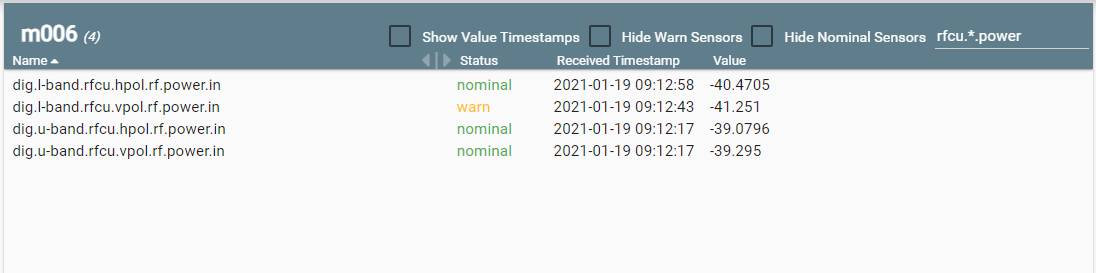
\includegraphics[scale=0.39]{Chapters/images/image83.png}
	
	%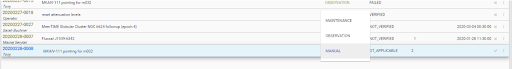
\includegraphics[resolution=100]{bur1.png}
	\caption{Global sync time remaining alert in sensor list}
	\label{fig:image83}
\end{figure}
The power levels for inputs on the L-band should be between -42dBm and -45dBm (when
not observing) and if they exceed these values this will be shown as warning. Low power
may mean that the LNA on the receiver are switched OFF or high power might mean AP is
pointing at a strong source or ground.\\

The second power level sensors for the digitisers are the ADC power levels which are
measured at the input of the ADC after the gains have been applied. The gains depends on
the attenuation levels which can be manually set, but we use separate scripts in setting and
refining attenuations. This is important to configure the attenuations so that all antennas
have the same output power levels. From the CAM GUI sensor list, filter for adc power i.e.
adc.*.power.in. \textbf{Figure}~\ref{fig:image51} shows the power levels for each polarisation of m006.
\begin{figure}[H]
	\centering
	%\includegraphicsdpi{100}{}{bur1.png}     
	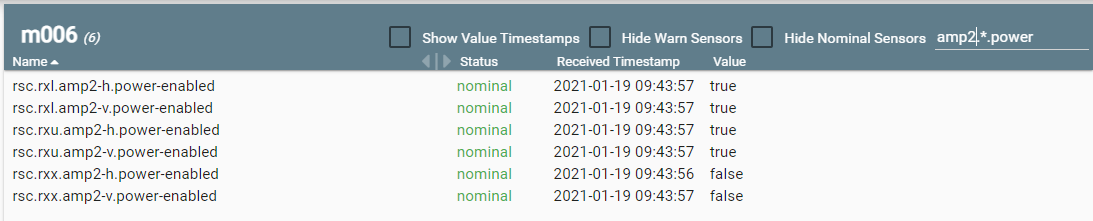
\includegraphics[scale=0.4]{Chapters/images/image51.png}
	
	%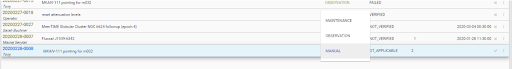
\includegraphics[resolution=100]{bur1.png}
	\caption{Global sync time remaining alert in sensor list}
	\label{fig:image51}
\end{figure}
It is recommended that the refine attenuations script should be run after building a new
subarray and the set attenuations script be run if there is a change in the signal chain i.e. a
Receiver or a Digitiser was replaced.
\section{ Updating config for a replaced digitiser}
Digitisers normally have their config files updated before they are handed over to
Operations. If a digitiser is replaced, it's serial number needs to be updated in CAM's
katconfig configuration files. This will require someone from the operations team to perform
github updates. The procedure to do that is shown below.\\

Note: Swaps done in S-band does not need updates in katconfig, because S-band
packetisers don’t use serial numbers, but instead use IP addresses according to the receptor number which gets set in the packetiser itself during installation.  This is their way
of communicating with MeerKAT. Hence the IP address never has to change when S-band
packetisers are replaced.
There are two different procedures which you can choose to follow:
\subsection{ On the terminal}
\begin{lstlisting}[style=DOS]
ssh kat@ops.kat.ac.za
cd katconfig/static/antennas/
git checkout master
git pull
git checkout karoo
git pull
git checkout -b update_m0XX_dig_config
\end{lstlisting}

If the response is:
\begin{lstlisting}[style=DOS]
fatal: A branch  named update\_m0XX\_dig_config already exists.
\end{lstlisting}
then rerun the command, but exclude “-b” this time.
\begin{lstlisting}[style=DOS]
git branch
\end{lstlisting}
 This should give: \option{*update\_m0XX\_dig\_config} 
\begin{lstlisting}[style=DOS]
ls
vi m0XX.conf 
\end{lstlisting}
(you can also use \option{nano m0XX.conf} whichever you comfortable with)

Type the letter “i” in order to edit the file.
The file format should be for example:
\begin{lstlisting}[style=DOS]
digitiser_l = ready:dig-041
\end{lstlisting} 
(we want to change this to the new serial number, i.e 064 for
example, to have \option{digitiser\_l = ready:dig-064})


any digitisers not installed should be of the format: 
\begin{lstlisting}[style=DOS]
digitiser_x = absent
\end{lstlisting}
Save the file and exit (press Esc, then type ":wq!")

\begin{lstlisting}[style=DOS]
git diff (shows changes you have made, check they are correct)
git add .
git commit -m "Updating (relevant band) digitiser serial no to 0XX on
m0XX"
git push --set-upstream origin update_m0XX_dig_config
\end{lstlisting}
\subsection{ On Github website}
\begin{itemize}


\item  Go to github:  \url{https://github.com/ska-sa/katconfig}
\item  Go to the new branch by clicking  on the dropdown list on available branches as shown in \textbf{Figure}~\ref{fig:image83} 
(should currently be on the karoo branch) and then selecting the branch name
of the new branch created .
\begin{figure}[H]
	\centering
	%\includegraphicsdpi{100}{}{bur1.png}     
	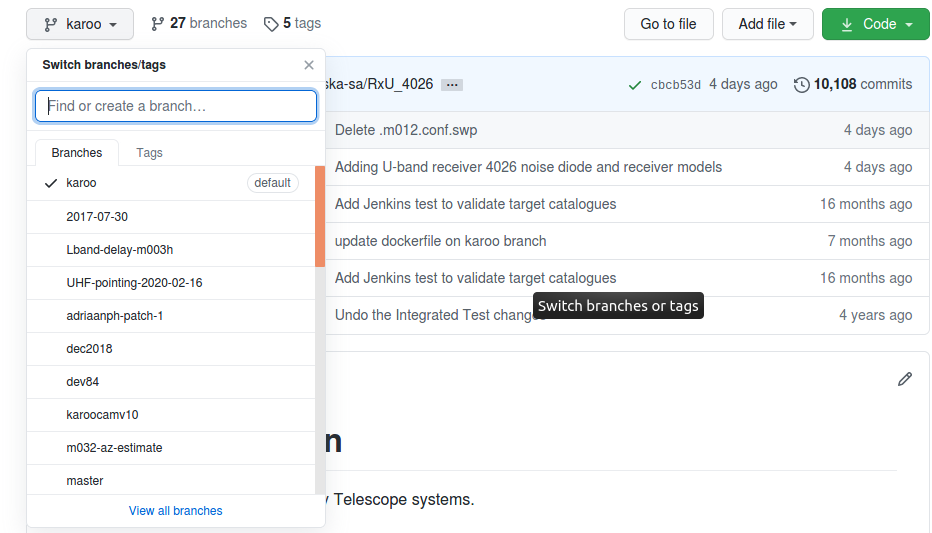
\includegraphics[scale=0.43]{Chapters/images/image108.png}
	
	%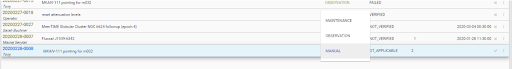
\includegraphics[resolution=100]{bur1.png}
	\caption{Github new branch select}
	\label{fig:image108}
\end{figure}

\item Create pull request from \option{update\_m0XX\_dig\_config} (name of branch created)
to karoo by clicking on “Pull request” at the top right as shown in \textbf{Figure}~\ref{fig:image73}.
\begin{figure}[H]
	\centering
	%\includegraphicsdpi{100}{}{bur1.png}     
	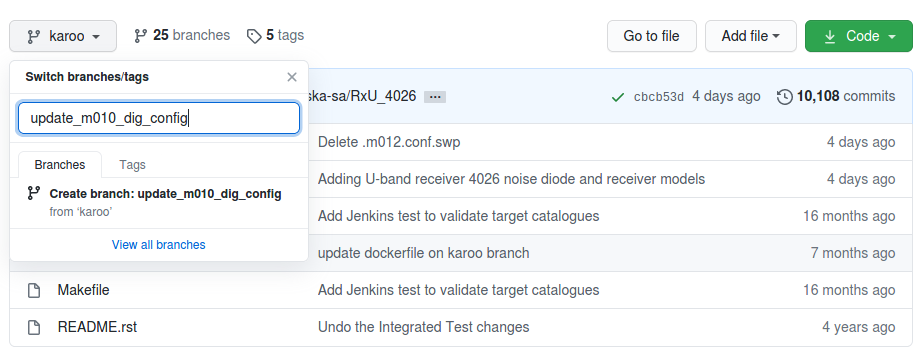
\includegraphics[scale=0.43]{Chapters/images/image73.png}
	
	%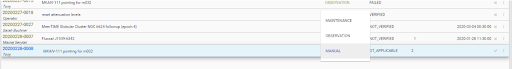
\includegraphics[resolution=100]{bur1.png}
	\caption{Github create pull request }
	\label{fig:image73}
\end{figure}



\item Make sure \option{base:karoo} and \option{compare:update\_m0XX\_dig\_config} is
selected. (Also make sure it’s only the files you have modified which are part
of the pull request - if you did the above steps properly that will be the case).
\item Then write a comment stating what you are doing, why (give Jira number if
applicable) and make the request out to Pieter Kotze. See an example in \textbf{Figure}~\ref{fig:image47}.
\begin{figure}[H]
	\centering
	%\includegraphicsdpi{100}{}{bur1.png}     
	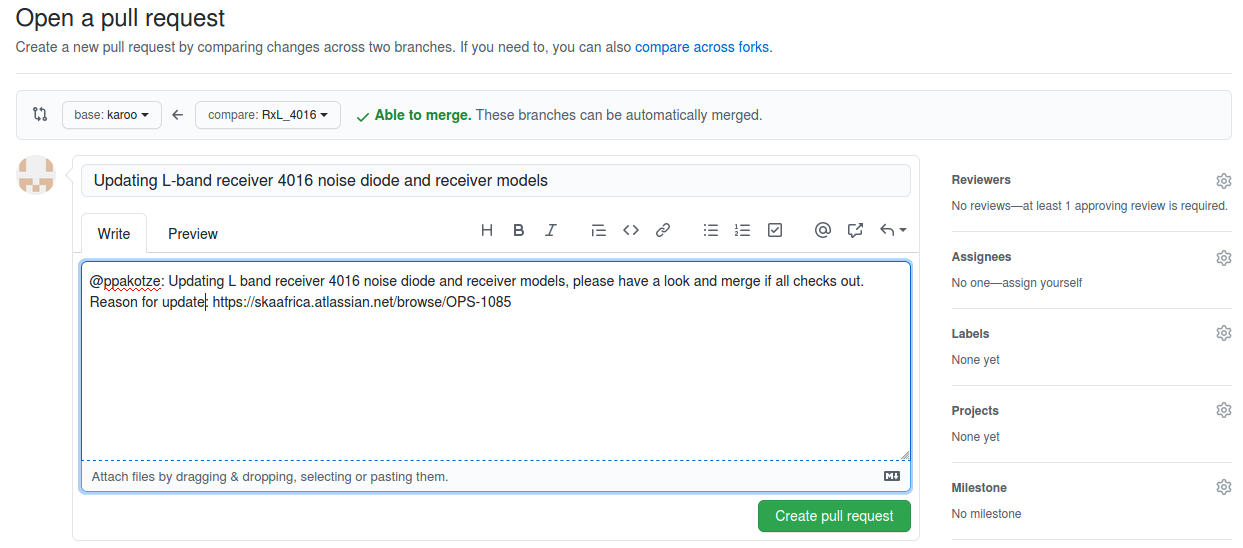
\includegraphics[scale=0.33]{Chapters/images/image47.png}
	
	%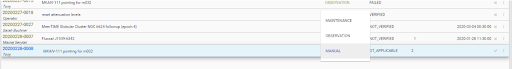
\includegraphics[resolution=100]{bur1.png}
	\caption{Github open pull request }
	\label{fig:image47}
\end{figure}
\item At the right hand side at the top next to “Reviewers”, click on the gear icon. It
will drop down a list of reviewers to choose from. Type “ppakotze” (see \textbf{Figure}~\ref{fig:reviewers}) in the
search field to find Pieter K and then click on Pieter K to request him to
approve your pull request (It will show a check mark next to his name, and
then under “Reviewers” you will see a yellow dot next to his name).

\begin{figure}[H]
	\centering
	%\includegraphicsdpi{100}{}{bur1.png}     
	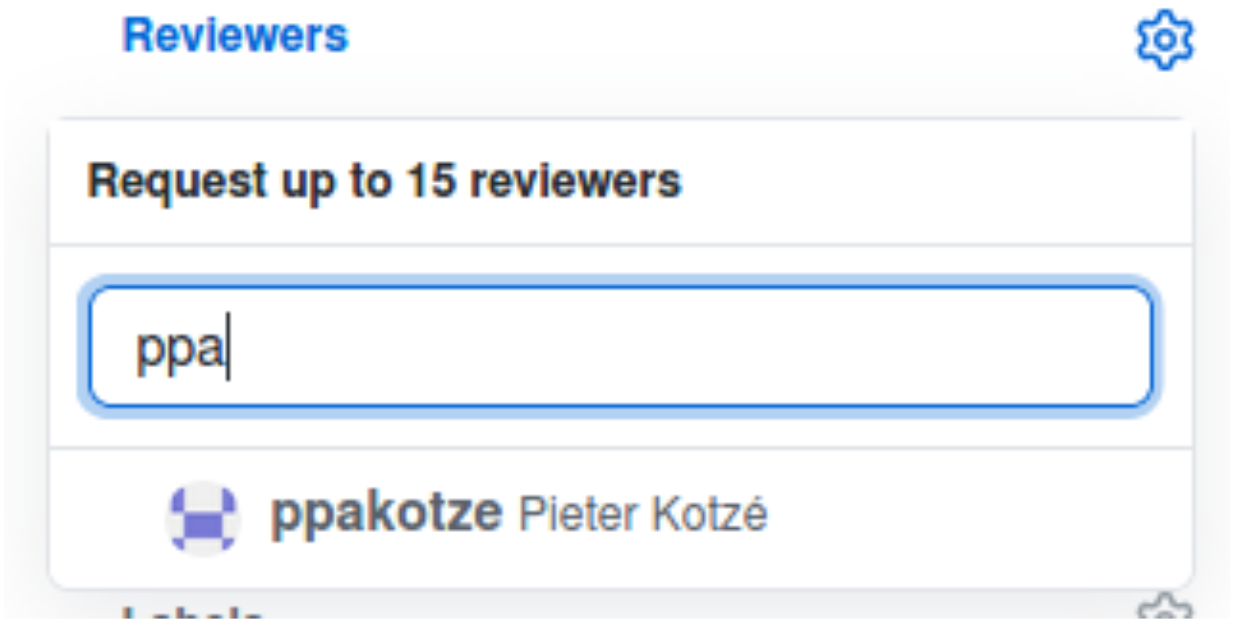
\includegraphics[scale=0.26]{Chapters/images/reviewers.png}
	
	%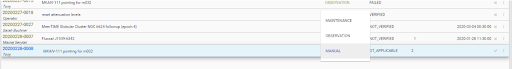
\includegraphics[resolution=100]{bur1.png}
	\caption{Github revievers dialogue }
	\label{fig:reviewers}
\end{figure}
\item Then click on “Create pull request”.\\
\textit{ Note: After Pieter K approves the pull request, he usually also merges
the pull request, but sometimes you have to do the merging yourself.
You do this by going to the pull request after it has been approved,
and then click on “Merge pull request” at the bottom and then “Confirm
merge”}
\end{itemize}






	
 
 \chapter{Chapter Three Title}
 
        The telescope system software runs on Linux servers and the basic understanding of the Linux operating system is required in order to operate the telescope. The Telescope Operator will also use Portal’s CAM graphical user interface referred to as GUI in order to interact with the telescope system. In order for anyone to interact with the telescope system, they need to have been given access via CAM portal.  The person needs a username and password to login into the system. When a person logs in for the first time on the system in order to control and monitor MeerKAT telescope system, the following is important to note. The system has many server nodes that are used for controlling and monitoring various parts of the system.  The most used servers nodes are:
        \begin{itemize}
\item{} \server{portal.mkat.karoo.kat.ac.za} and
\item{} \server{obs.mkat.karoo.kat.ac.za} 
\end{itemize}
The naming convention for the server nodes is always\\ $<$\server{server}$>$.$<$\server{telescope}$>.<$\server{site}$>$\server{.kat.ac.za.}, with :
\begin{itemize}
\item{} the first parameter is server node name
\item{} the second is the telescope (Currently: \server{mkat, kat7, mkat-rts}) and
\item{} the third is karoo for site systems different from lab systems.
\end{itemize}
\subsection{Portal Server}
The URL of where to find the GUI is \server{http://portal.mkat.karoo.kat.ac.za/}. 
The login details to the portal link above will be provided by CAM admistrator.
The landing page is as shown in \textbf{Figure}~\ref{fig:image71}. 
\clearpage
\begin{figure}[!thb]
	\centering
	%\includegraphicsdpi{100}{}{bur1.png}     
	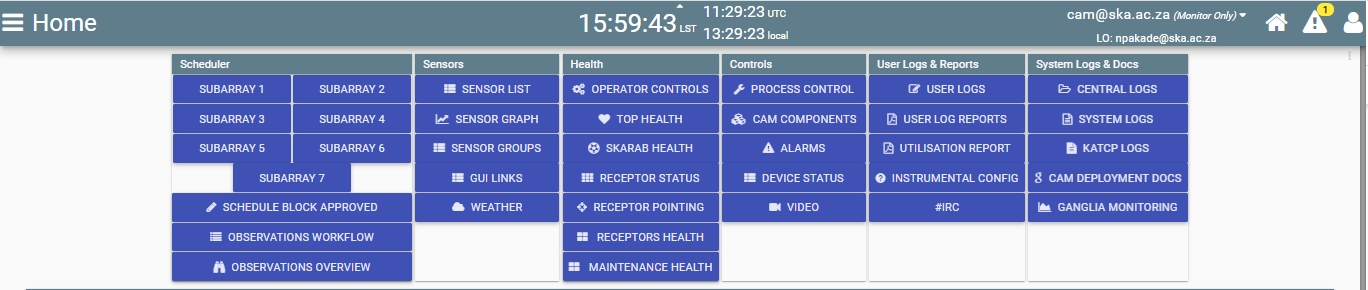
\includegraphics[scale=0.3]{Chapters/images/image71.png}
	
	%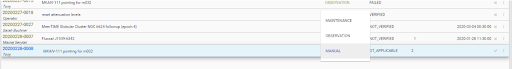
\includegraphics[resolution=100]{bur1.png}
	\caption{CAM GUI home page}
	\label{fig:image71}
\end{figure}




This will allow one to monitor the telescope system but will not be able to control the system. The person will have to be given the lead operator role (LO) or expert role in order to control the telescope for safety reasons. This page will allow one to access different functionality of the telescope system, monitoring and control i.e. if for instance one is interested in building and running subarray 1, the configuring of a subarray, one will click and open “SUBARRAY1 tab. This page will be shown as in \textbf{Figure}~\ref{fig:image38} below.

\begin{figure}[!thb]
	\centering
	%\includegraphicsdpi{100}{}{bur1.png}     
	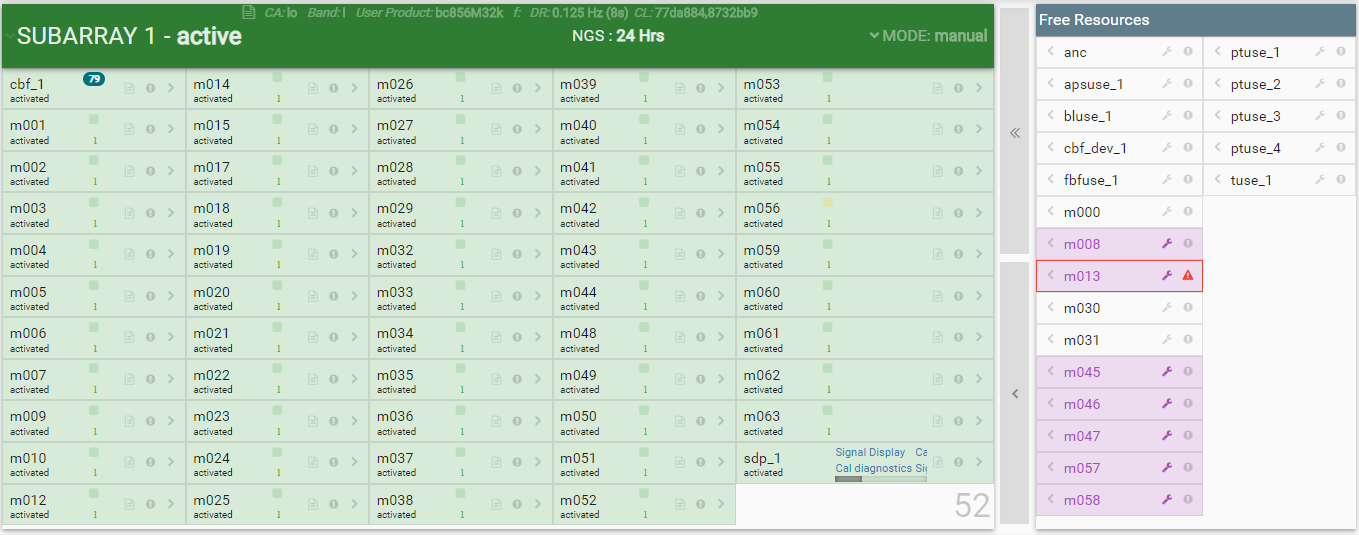
\includegraphics[scale=0.3]{Chapters/images/image38.png}
	
	%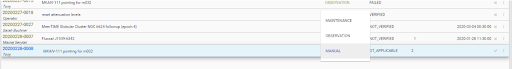
\includegraphics[resolution=100]{bur1.png}
	\caption{CAM GUI Subarray1 window}
	\label{fig:image38}
\end{figure}




In order to learn more about the GUI and the telescope system, the user must familiarise with different tabs on the GUI. More information will be discussed in the following sections of this document. 

\subsection{Obs Server/Machine}
The node server \server{“obs.mkat.karoo.kat.ac.za”} allows interaction with the live system via the command line and ipython interface. This is where the instructions to create a schedule block SB is provided.The user is required to command the telescope in the Linux environment from the command line using Linux and python commands. 
\clearpage
The user will be given credentials to login into the server. The server node to login using ssh command is \server{“obs.mkat.karoo.kat.ac.za” } and this will open up a page as shown in \textbf{Figure}~\ref{fig:image87}.

%\begin{figure}[!thb]
%	\centering
%	%\includegraphicsdpi{100}{}{bur1.png}     
%	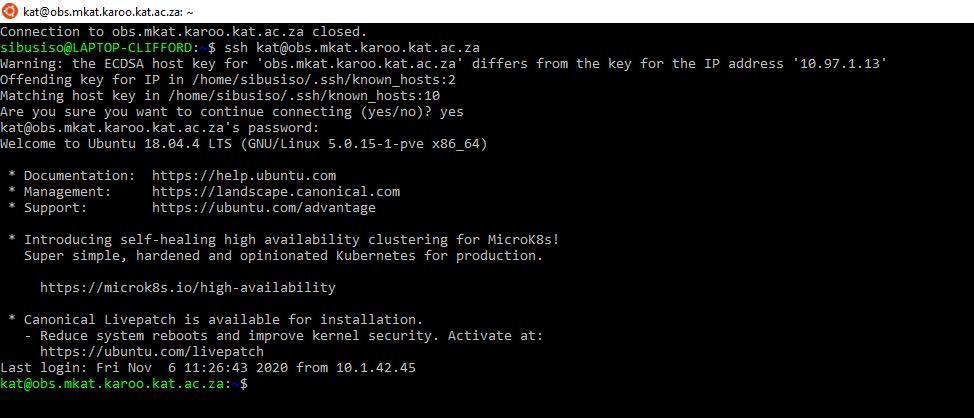
\includegraphics[scale=0.45]{Chapters/images/image87.png}
%	
%	%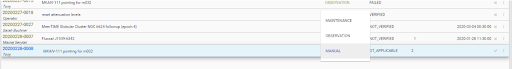
\includegraphics[resolution=100]{bur1.png}
%	\caption{Terminal ssh login to obs machine}
%	\label{fig:image87}
%\end{figure}
\begin{figure}[!thb]
	\centering
	%\includegraphicsdpi{100}{}{bur1.png}     
	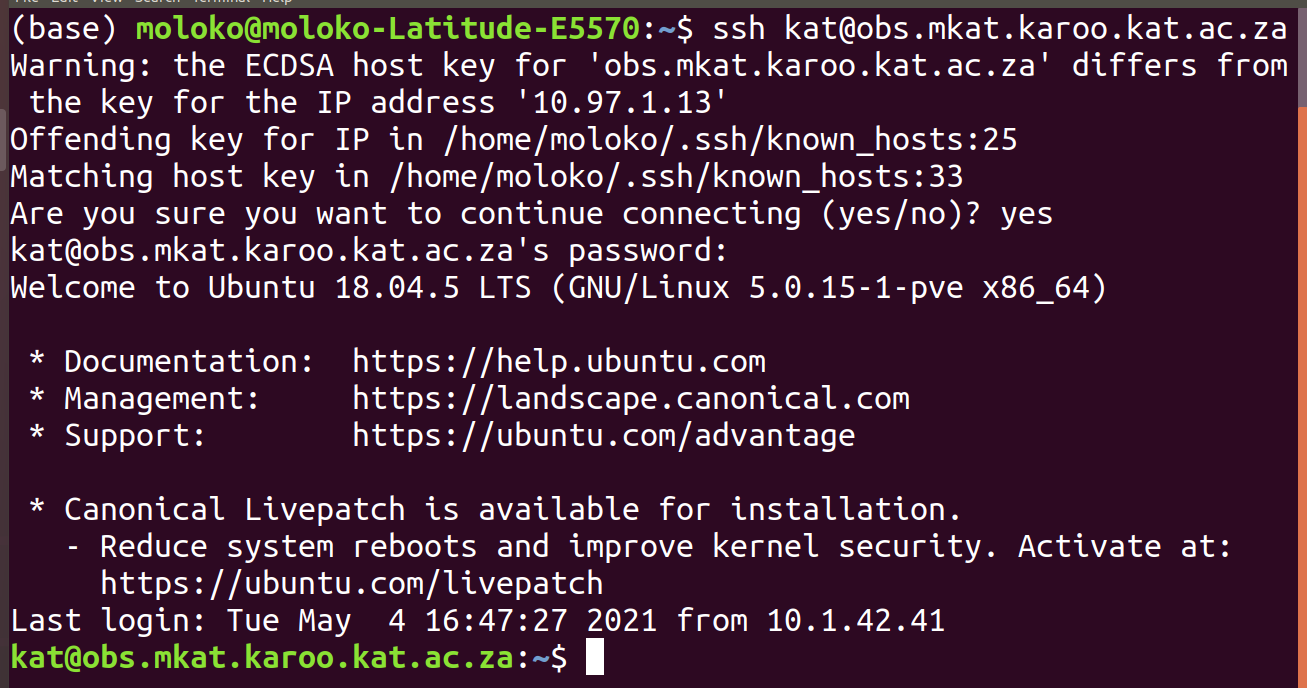
\includegraphics[scale=0.33]{Chapters/images/terminal.png}
	
	%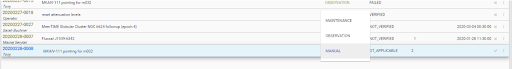
\includegraphics[resolution=100]{bur1.png}
	\caption{Terminal ssh login to obs machine}
	\label{fig:image87}
\end{figure}
 
 \chapter{Chapter Four Title}
  

The telescope can only be controlled by a lead operator who has the correct credentials. To be a lead operator you will have credentials to control and monitor the telescope and these credentials are supplied by the Telescope Operations Manager. The telescope operates 24 hours a day, 7 days week and 365 days a year and there are 3 shifts a day split over 8 hours each. During the shift we have a lead operator who is responsible for controlling and monitoring the telescope system. Therefore there are three operators over a 24 hour period configuring and monitoring the telescope system at all times. Between the shifts one lead operator  hands over the system to the next operator. The paragraphs below describe in detail the procedure begging followed during the handover process.  
\section{Operator Handover Procedures}
Each Operator during the shift compiles a list or record  of the incidents that occured during  shift.  This record is called a handover document and this is different from the operations meeting minutes. The operator will update the incoming lead operator and also give this document to the next lead operator and this document will contain but not limited to this information below:
\begin{itemize}
\item{} What is currently being done with the telescope?
\item{} What observation is coming up after the current one?
\item{} What receptors are available and what receptors are expected back from maintenance?
\item{} What resources have been booked out for. maintenance and when - who to contact to get them back?
\item{} What problems are currently opened under which subsystems - supplement? this with reading open-ended user logs and the checklist [\textbf{Appendix A}]"
\item{} What are the problems experienced and what does the incoming operator need to look out for?
\end{itemize}
\section{Booking resource for maintenance}
The lead operator during the morning shift will be required to make resources (AP, Receivers, Digitiser, CBF etc) available to site technicians and engineers to conduct maintenance and upgrades. The resources will normally be booked for maintenance or upgrade at least a day before unless the resource is in error and cannot be used for operations. The lead operator will follow the process below:
\begin{itemize}
\item{} Check for booking in the Engineering Spreadsheet or Site calendar.
\item{} Mark the resource to maintenance - a log is automatically opened in the user logs. Add reason for booking in the log.
\item{} If the resource booked causes system downtime, add the ‘timeloss’ tag to the user log for system utilisation statistics reporting.
\item{} Alert maintenance staff or engineering staff after the resources have been made available. 
\item{} This information must also be added in the handover document. 
\end{itemize}
\section{ Receiving a resource after maintenance or an update}
\begin{itemize}
\item{} During the handover, check the control status of the resource \sensor{ap.control} sensor in sensor list  as shown in \textbf{Figure}~\ref{fig:image98}.

 \begin{itemize}
\item[$\circ$] If it is in remote - usable
\item[$\circ$] If it is in local/manual/e-stop - must be reset by technician
\end{itemize}

\begin{figure}[!thb]
	\centering
	%\includegraphicsdpi{100}{}{bur1.png}     
	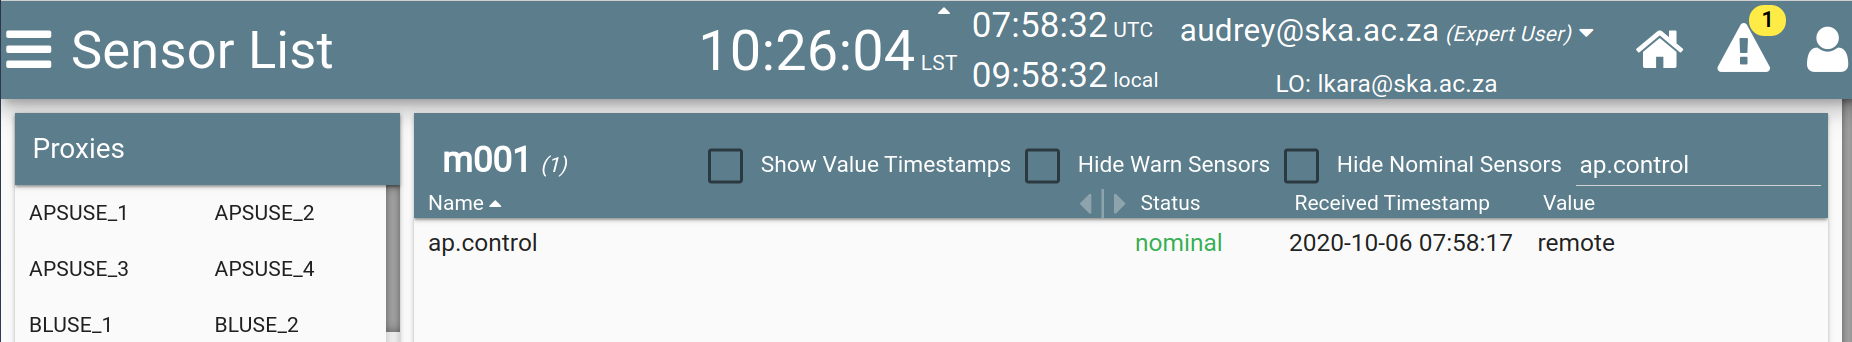
\includegraphics[scale=0.25]{Chapters/images/image98.png}
	
	%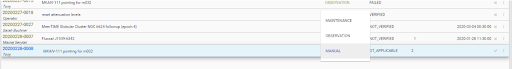
\includegraphics[resolution=100]{bur1.png}
	\caption{CAM GUI sensor list filtered with "Control"}
	\label{fig:image98}
\end{figure}
\item{} If in remote, check the health of the resource in detail

\begin{lstlisting}[style=DOS]
ssh kat@obs.mkat.karoo.kat.ac.za
./katsdpscripts/utility/check_ant.py --observer name --ant m0xx --proposal-id 22

\end{lstlisting}

Or 
\begin{lstlisting}[style=DOS]
./usersnfs/tiyani/meerkat_status.py --receiver rxl     

\end{lstlisting} (For L-band receivers)
\begin{lstlisting}[style=DOS]

./usersnfs/tiyani/meerkat_status.py --receiver rxu     

\end{lstlisting}
 (For UHF receivers)


\item{} Include the AP in the next observation to check signal quality
\item{} If a number of antennas are returning from maintenance and there is time before the next observation, create a small subarray with at least 4 antennas and run delay calibration, if there are less than 4 antennas available, build a subarray with those antennas but run three calibration script to check signal health.
\item{} Update OPS Catalyst page with correct number of APs available for use.

\section{Integrating a Receptor into Meerkat}
This must be done when an antenna has been in maintenance for an extended period of time or it was handed over to MPI for testing

Verify with the person who took the AP if they have changed anything in the digitiser,receiver or any other component configuration.
If there were changes made, talk to CAM to change what has been changed before testing the AP.
Run the \file{"check\_ant.py”} script as in the step above in 6.2
Mark the digitiser ready 
\begin{lstlisting}[style=DOS]
ssh kat@obs.mkat.karoo.kat.ac.za
ipython			
import katuilib
configure_cam("camcam","all")
cam.m0xx.sensor.dig`_selected_band.get_value()
cam.m0xx.req.digitiser_ready('l', timeout=60)
cam.m0xx.req.dig_select_band('l', timeout=60)
\end{lstlisting}




Where \component{m0xx} represents a receptor number e.g \component{m001}

\item{} Sync the digitiser using global sync - see next chapter.
\item{} Check the remaining hours left before the next global sync in sensor list of the CAM GUI as shown in \textbf{Figure}~\ref{fig:image68}.


\begin{figure}[!thb]
	\centering
	%\includegraphicsdpi{100}{}{bur1.png}     
	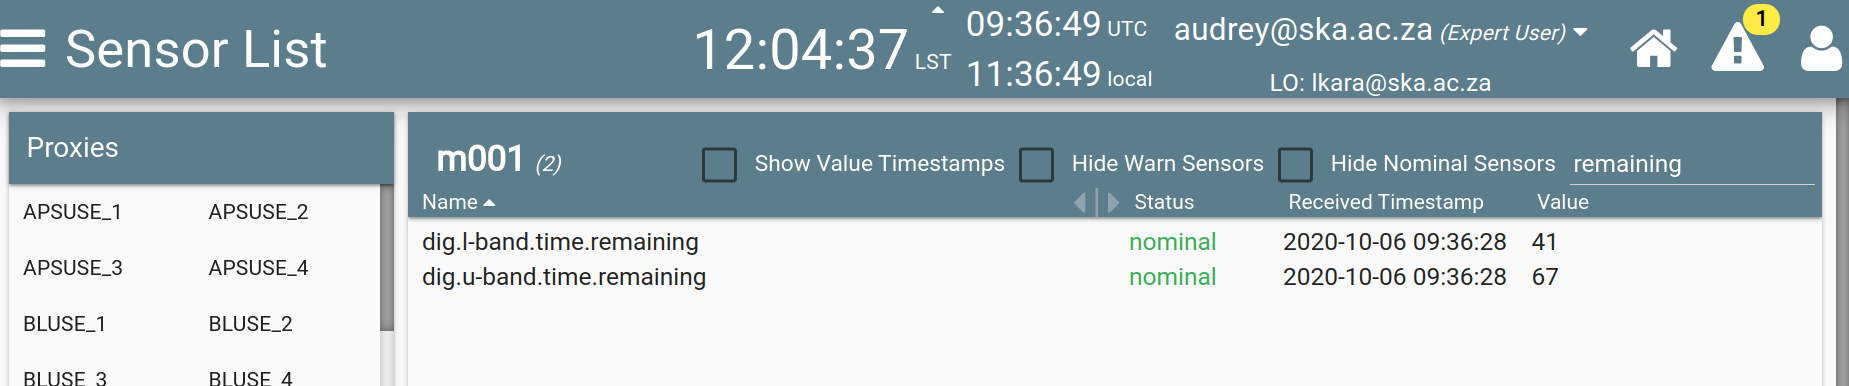
\includegraphics[scale=0.25]{Chapters/images/image68.png}
	
	%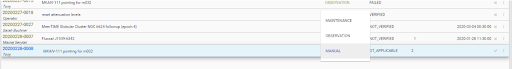
\includegraphics[resolution=100]{bur1.png}
	\caption{CAM GUI sensor list filtered by "remaining".}
	\label{fig:image68}
\end{figure}

These values above (41 \& 67) will indicate if global sync was successful or not for L and UHF$-$band digitisers.

\item{} Include the antenna in an array and run a calibrated delay script and see if it finds a solution. 
\begin{itemize}
\item [$\circ$] Look at the progress output of the delay cal script if the delay solutions are found.
		\item [$\circ$] During observation, look at the waterfall plot(signal displays) to see if there is a constant colour on its baseline. If the antenna looks noisy as in \textbf{Figure}~\ref{fig:image34} or has a rainbow, ask AoD to check its delay models.
\end{itemize}
 

\begin{figure}[!thb]
	\centering
	%\includegraphicsdpi{100}{}{bur1.png}     
	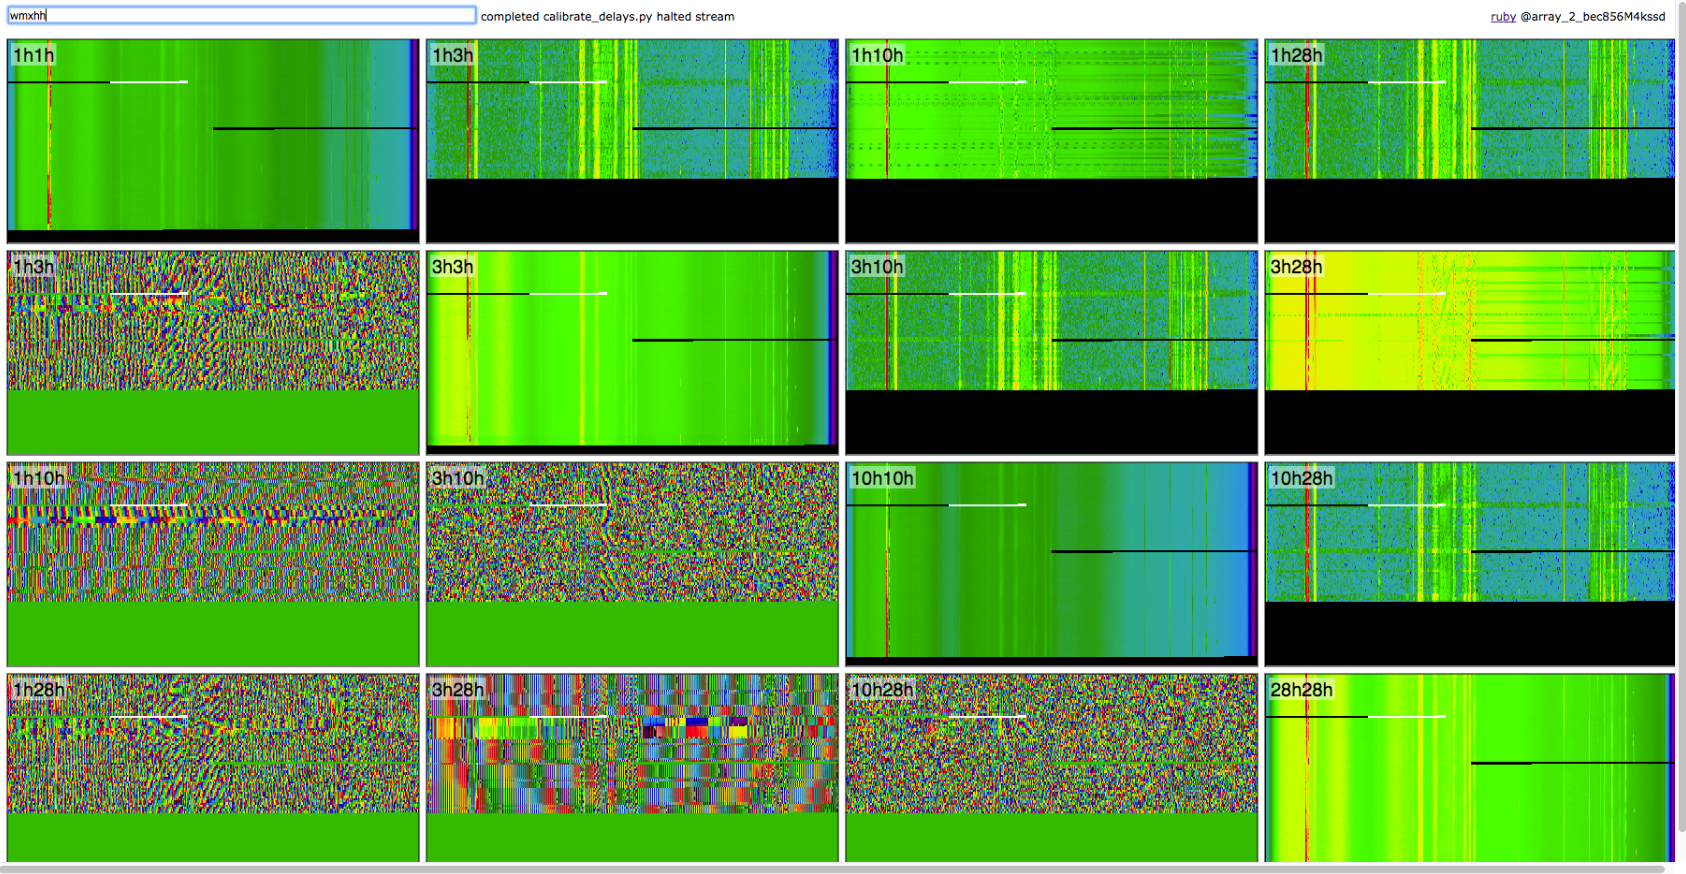
\includegraphics[scale=0.25]{Chapters/images/image34.png}
	
	%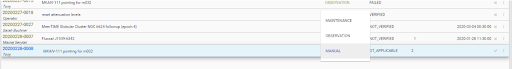
\includegraphics[resolution=100]{bur1.png}
	\caption{SDP waterfall plot.}
	\label{fig:image34}
\end{figure}

\item{} Before including the antenna in a Science observation communicate with the AoD about:
\begin{itemize}
	\item [$\circ$] interferometric pointing and notify operators to update pointing and delay models.
\end{itemize}

\item{} Update the Engineering Meerkat spreadsheet in the Owner tab.
\item{} Update the associated jira if necessary and close it.
\end{itemize}
 
 \chapter{Conclusion}
 \input{Chapters/conclusion}
 \appendix
 \chapter{Appendix Title}
 \begin{itemize}


\item[] \textbf{Starting your shift:}

\begin{table}[H]
	
	\label{tab:checklist}
	\begin{tabular}[b]{|p{16 cm}|} 
		\hline
 Did you read the handover on OPS-CATALYST?\\
\hline
Did you read the Notice board?\\
\hline
Have you reserved antennas for site maintenance?\\
\hline
Will the sync epoch time suffice for the current schedule block?\\
\hline
Have you opened mattermost communications tool.\\
\hline
Did you run AP Meerkat status script to check availability of AP?\\
\hline
	
	\end{tabular}
\end{table}

 


\item[] \textbf{Subarray Configurations:
}
\begin{table}[H]
	
	\label{tab:checklist}
	\begin{tabular}[b]{|p{16 cm}|} 
		\hline
	Is the band, data product,dump rate,cbf,sdp and USE as per calendar request?\\
	\hline
	Have you run reset attenuation after adding antennas from maintenance?\\
	\hline
	Have all antennas calibrated for delays? if not, repeat and/or mark faulty ones?\\
	\hline
	Have you verified if phase-up must be run from calendar request?\\
	\hline
	
		
	\end{tabular}
\end{table}


 
 

\item[] \textbf{Observation:
}
\begin{table}[H]
	
	\label{tab:checklist}
	\begin{tabular}[b]{|p{16 cm}|} 
		\hline
 Is the dryrun valid, if not consult AOD\\
	\hline
	Are signal displays plotting?\\
	\hline
	
	Do you follow the progress report of the observation\\
	\hline
	Are observation files closed without errors\\
	\hline
	Is the observation file in the archive?\\
	\hline
	Have you checked the cal report and conducted the QA?\\
	\hline
	Have you opened JIRAs for encountered system problems?\\
	\hline
	Have you created/closed any timeloss logs on the telescope?\\
	\hline
	Have you updated the observation document and Operations Minutes?\\
	\hline
	
	
	Have you updated the Ops catalyst with the number of antennas available?\\
	\hline
		
	\end{tabular}
\end{table}
\end{itemize}

 \begin{itemize}


\item[] \textbf{Starting your shift:}

\begin{table}[H]
	
	\label{tab:checklist}
	\begin{tabular}[b]{|p{16 cm}|} 
		\hline
 Did you read the handover on OPS-CATALYST?\\
\hline
Did you read the Notice board?\\
\hline
Have you reserved antennas for site maintenance?\\
\hline
Will the sync epoch time suffice for the current schedule block?\\
\hline
Have you opened mattermost communications tool.\\
\hline
Did you run AP Meerkat status script to check availability of AP?\\
\hline
	
	\end{tabular}
\end{table}

 


\item[] \textbf{Subarray Configurations:
}
\begin{table}[H]
	
	\label{tab:checklist}
	\begin{tabular}[b]{|p{16 cm}|} 
		\hline
	Is the band, data product,dump rate,cbf,sdp and USE as per calendar request?\\
	\hline
	Have you run reset attenuation after adding antennas from maintenance?\\
	\hline
	Have all antennas calibrated for delays? if not, repeat and/or mark faulty ones?\\
	\hline
	Have you verified if phase-up must be run from calendar request?\\
	\hline
	
		
	\end{tabular}
\end{table}


 
 

\item[] \textbf{Observation:
}
\begin{table}[H]
	
	\label{tab:checklist}
	\begin{tabular}[b]{|p{16 cm}|} 
		\hline
 Is the dryrun valid, if not consult AOD\\
	\hline
	Are signal displays plotting?\\
	\hline
	
	Do you follow the progress report of the observation\\
	\hline
	Are observation files closed without errors\\
	\hline
	Is the observation file in the archive?\\
	\hline
	Have you checked the cal report and conducted the QA?\\
	\hline
	Have you opened JIRAs for encountered system problems?\\
	\hline
	Have you created/closed any timeloss logs on the telescope?\\
	\hline
	Have you updated the observation document and Operations Minutes?\\
	\hline
	
	
	Have you updated the Ops catalyst with the number of antennas available?\\
	\hline
		
	\end{tabular}
\end{table}
\end{itemize}

 
\bibliographystyle{plain}
\bibliography{references} 
\end{document}